\begin{frame}
	\frametitle{Curve Ellittiche}

\begin{columns}
	\begin{column}{.65\textwidth}

		\begin{itemize}
			\item curve definite su un certo $\mathbb{F}_\orange{q}$ da 
				$$y^2=x^3+\orange{a}x+\orange{b}$$
			\item non singolari, \textit{i.e.} $4a^3+27b^2\neq 0$
		\end{itemize}

		\begin{theorem}[Hasse]
			 sia $\mathbb{F}_q$ il campo di Galois di ordine $q$ 
			 \newline sia $\mathcal{E}_q=\mathcal{E}_{(a,b)}(\mathbb{F}_q)$ una sua curva ellittica 
			\vspace*{4pt}
			\begin{enumerate}
				\item $|o(\mathcal{E}_q)-(q+1)|\leq2\sqrt q$
			\end{enumerate}	
		\end{theorem} 
		$\;\;\;\Rightarrow\;\;${\color{blue}ordine} \textit{GF} governa \textit{difficoltà}

	\end{column}

	\begin{column}{.4\textwidth}
		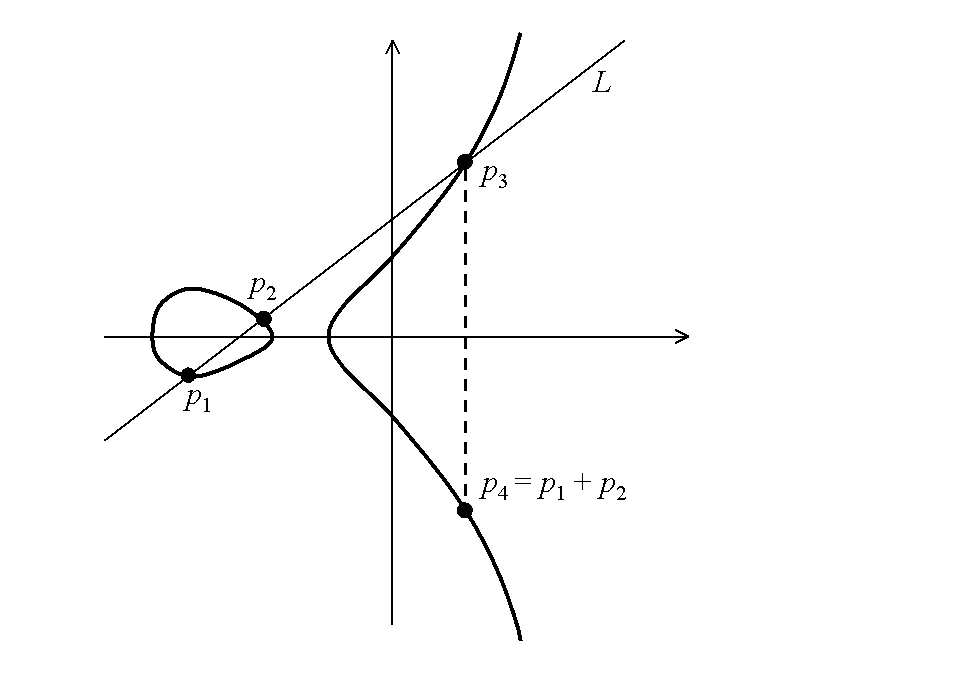
\includegraphics[height = 5 cm]{images/eca.png}
	\end{column}
\end{columns}

\end{frame}
%-------------------------------------------------------------------------
\begin{frame}
	\frametitle{Curve Ellittiche}
	\framesubtitle{legge di gruppo: definizione}
	
	$(\mathcal{E}_{(a,b)}(\mathbb{F}_q),\; \red{+})$ definisce un {\color{blue}gruppo abeliano}
	$$ \orange{R} = \orange{P}+\orange{Q} \triangleq(\orange{x_R},\,{\color{red}-}\orange{y_R}) $$
	$$x_P \neq x_Q \;: \;\;
  			\left \{ \begin{array}{lr}
	  			y_R \triangleq y_P+s(x_R-y_P) \\
				x_R \triangleq s^2-x_P-x_Q & s=\frac{y_P-y_Q}{x_P-x_Q}
			\end{array} \right. $$
			
	$$x_P = x_Q \;: \;\;
  			\left \{ \begin{array}{lcr}
 
  			y_P = -y_Q\;: & R = O \\
			 y_P = y_Q \neq 0\;: & \left\{
				  \begin{array}{lcr}
				  	y_R \triangleq y_P+s(x_R-y_P) \\
				    x_R \triangleq s^2-2x_P & s=\frac{3x_P^2+a}{2y_P}
				  \end{array}
				\right. 
			\end{array} \right. $$
 	\vspace{1pt}				
 	$$ \orange{R} = \orange{P}{\color{red}\times}\orange{n} 
 		\triangleq \orange{P}+\orange{P}+\ldots+\orange{P}\;\;\;\;\;\;\;\;\; n\in \mathbb{Z}\;\;\mathrm{volte}$$
	
\end{frame}
%-------------------------------------------------------------------------
\begin{frame}
\frametitle{Curve Ellittiche}
	\framesubtitle{legge di gruppo: casistica}
	
	\begin{figure}[H]
	 	\begin{center}
			 \begin{tabular}{c @{\hspace{1em}} c}
				 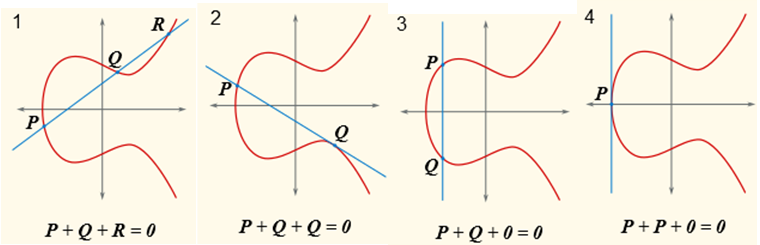
\includegraphics[width = 11 cm]{images/ecalgebrarow.png}
			 \end{tabular}
		 \end{center}
 	\end{figure}
	
\end{frame}	
%-------------------------------------------------------------------------
\begin{frame}
	\frametitle{Curve Ellittiche}
	\framesubtitle{problema matematico}
	
	%$(\mathcal{E}_{(a,b)}(\mathbb{F}_q),\,+)$ è un gruppo abeliano
% 	\begin{itemize}
% 		\item chiusura
% 		\item associatività
% 		\item identità %SAY come visto prima
% 		\item invertibilità %SAY come visto prima
% 		\item commutatività
% 	\end{itemize}  
	
	trovare un segreto ${\color{red}d}\in[1,\,n-1]$, dati
	\begin{itemize}
	  \item $\orange{\mathcal{E}}=\mathcal{E}_{(a,b)}(\mathbb{F}_q)$
	  \item $\orange{G}\in \mathcal{E}:\;\;\;\;\;\;\tiny{<}\,G\,\tiny{>}=\mathcal{E}$
	  \item $\orange{n}=o(G):\;G\times n= O=P_\infty$, $\;\;	\;n\;$ primo
	  \item $\orange{P}\in \mathcal{E}$
	  \item $\orange{Q}=P\times d$
	\end{itemize}
\end{frame}